\documentclass[10pt,a4paper,landscape]{article}

% -- Layout ----
\usepackage[top=0.25cm, bottom=0.25cm, left=0.25cm, right=0.25cm, landscape]{geometry}

% -- Titles ----
\usepackage[
  tiny,                     % text size title
  compact                   % reduce vertical space before/after title
]{titlesec}
% \titlespacing*
% \titleformat{\section}{\normalfont\Large\bfseries}{\thesection}{0em}{} % Remove space before and after section titles
% \titleformat{\subsection}{\normalfont\large\bfseries}{\thesubsection}{0em}{} % Remove space before and after subsection titles

\titlespacing*{\section}{0pt}{0pt}{0pt} % Remove space before/after section titles
\titlespacing*{\subsection}{0pt}{0pt}{0pt} % Remove space before/after subsec titles

% -- Colors ----
\usepackage[dvipsnames]{xcolor}

% -- Math ------
\usepackage{mathtools}
\usepackage{amssymb}
\usepackage{turnstile}%better vdash
% -- Lists -----
\usepackage[inline]{enumitem}
\setlist{noitemsep}% Remove vspace between items
% Set vspace before and after  list environments as well as the left margin
\setlist[itemize,1]{leftmargin=*,labelindent=1pt,topsep=1pt,partopsep=1pt}
\setlist[itemize,2]{leftmargin=2pt,topsep=1pt,partopsep=1pt}
\setlist[enumerate,1]{leftmargin=*,labelindent=1pt,topsep=1pt,partopsep=1pt}
\setlist[enumerate,2]{leftmargin=2pt,topsep=1pt,partopsep=1pt}

% -- Code listing ---
\usepackage{listings}
\lstset{
  aboveskip=3pt,
  belowskip=3pt,
  basicstyle=\small\ttfamily,
  commentstyle=\upshape\ttfamily,
  frame=single,
  language=Haskell,
}

% Parse Trees
\usepackage{tikz}
\usetikzlibrary{ arrows, automata, bbox, positioning}
\tikzset{
->, % makes the edges directed
>=stealth', % makes the arrow heads bold
node distance=1cm, % specifies minimum distance between two nodes
smallnode/.style={},
every state/.style={thick}, % sets the properties for each ’state’ node
initial text=start, % sets the text that appears on the start arrow
}

% Place a figure env right here via [H] option
\usepackage{float}

% Side by side figure
\usepackage{subcaption}

% -- Multi Columns --
\usepackage{multicol}

% -- Global spacing settings ----
\setlength{\abovedisplayskip}{3pt}
\setlength{\belowdisplayskip}{3pt}
\setlength{\abovedisplayshortskip}{3pt}
\setlength{\belowdisplayshortskip}{3pt}
\setlength{\parindent}{0pt}
\setlength{\parskip}{0pt plus 0.5ex}

\begin{document}
% Suppress page number for all pages
\pagestyle{empty}

\begin{multicols*}{3}
\section*{Hoare logic}
% Find the \textbf{weakest precondition} (most general).\\
\textbf{Weakest} possible: \textbf{\texttt{True}} \\
\textbf{Strongest} possible: \textbf{\texttt{False}} \\
\textbf{Strong} pre/post-conditions: more \textbf{specific} (say \emph{more}) \\
\textbf{Weaker} pre/post-conditions: more \textbf{general} (say \emph{less})

\subsection*{1/6 Assignment Rule}
\subsubsection*{Question Type 1}
Given post-condition \& one single assignment, ask for pre-condition:
\(\{?\}\,S\,\{Q\}\)

For example: \(\{?\}\ i := 2 * i \{i < 6\}\)

\textbf{Solution}
\begin{enumerate}
\item \textbf{Copy} Q over to P: \(\{i_{post} < 6\}\)
\item Replace all LHS vars with RHS vars: \(\{2 * i_{orig} < 6\}\)
\item See if any math/logic equivalence (simplify P if possible): \(\{i_{orig} < 3\}\)
\end{enumerate}

\subsubsection*{Question Type 2}
Prove the given Hoare Triple: \(\{P\}\,V := E\,\{Q\}\)

For example: \(\{x > 3\}\;x:=x+2\;\{x>5\}\)
\textbf{Solution}
\begin{enumerate}
\item \textbf{Copy} Q over to P: \(\{x_{post} > 5\}\)
\item Replace all LHS vars with RHS vars: \(x_{assign}+2 > 5\}\)
\item See if any math/logic equivalence (simplify P if possible): \(\{x_{orig} > 3\}\)
\end{enumerate}



\subsection*{2/6 Pre-condition Strengthening}

Logic: \(P_{strong} \rightarrow P_{orig} \)
\begin{displaymath}
  \frac{P_{strong} \rightarrow P_{weak} \quad \{P_{weak}\}\,S\,\{Q\} } {\{P_{s}\}\,S\,\{Q\}}
\end{displaymath}

\subsection*{3/6 Post-condition Weakening}
Logic: \(Q_{orig} \rightarrow Q_{weak} \)
\begin{displaymath}
  \frac{Q_{strong}\rightarrow Q_{weak} \quad \{P\}\,S\,\{Q_{strong}\} } {\{P\}\,S\,\{Q_{w}\}}
\end{displaymath}

\subsection*{4/6 Sequencing}
\subsubsection*{Question Type}
{
  % Reducing vertical spacing
  \setlength{\abovedisplayskip}{0pt}
  \setlength{\belowdisplayskip}{3pt}
  \setlength{\abovedisplayshortskip}{0pt}
  \setlength{\belowdisplayshortskip}{3pt}

  \[\textbf{Prove:}\quad \{P\}\,S_{1};\,S_{2};\,\ldots ;\,S_{n}\,\{Q\}\]
}
\textbf{Solution} Start backwards and use Assignment Rule:
\begin{enumerate}
\item\label{step1} \textbf{Copy} \(Q_{n}\) as \(P_{n}\) for \(S_{n}\)
\item\label{step2} \textbf{Use} assignment rule and math equivalence to simplify \(P_{n}\) if possible
\item \textbf{Use} \(P_{n}\) as \(P_{n-1}\) for \(S_{n-1}\)
\item \textbf{Repeat} \ref{step1} and \ref{step2} until getting \(P_{1}\)
\item \textbf{Strengthen} precondition \(\{P\}\rightarrow \{P_{1}\}\)
\item (Optional) Sometimes need (0th/boolean) logic to simplify compound propositions.

\end{enumerate}

\subsection*{5/6 Conditionals}
\subsubsection*{Question Type}
{
  % Reducing vertical spacing
  \setlength{\abovedisplayskip}{0pt}
  \setlength{\belowdisplayskip}{3pt}
  \setlength{\abovedisplayshortskip}{0pt}
  \setlength{\belowdisplayshortskip}{3pt}

\[\textbf{Prove:}\quad \{P\}\;if\:b\:then\:S_{1}\:else\:S_{2}\;\{Q\}\]
}
\textbf{Solution} Use Conditional Rule to prove both:
\begin{description}
\item [premise1] \(\{P \land b\}\:S_{1}\:\{Q\}\)
\item [premise2] \(\{P \land \neg b\}\:S_{2}\:\{Q\}\)
\end{description}
For each premise:
\begin{enumerate}
\item\label{step1} \textbf{Use} Assignment rule to get new \(P_{assign}\)
\item\label{step2} \textbf{Use} Propositional logic, math (precondition equivalence) to \textbf{strengthen} the \(P_{assign}\) for \(P_{s}\) (which is the \(P\) needed in the premise1)
\end{enumerate}
Then \textbf{use} Conditional Rule to combine the proved premises.

\subsubsection*{Complete conditionals}
Conditionals with \texttt{else} branch are \emph{complete}.

\texttt{if b then S} $\Longleftrightarrow$ \texttt{if b then S else (do nothing)}
\begin{displaymath}
  \frac{\{P \land\; b\}\;S\{Q\} \quad \{P \land \;\neg b\}\;\texttt{(do nothing)}\;\{Q\}}{\{P\}\;if\;b\;then\;S\;\{Q\}}
\end{displaymath}
\texttt{do nothing} can be \textbf{strengthened} to sth like \verb|x := x|

\section*{DFA}
Any \(S_{curr}\) has ONLY ONE transition to next \(S_{next}\)
\section*{NFA}
A \(S\) can have MANY transitions to next \(S_{n}\)
\section*{Regex}
\section*{Context-free Language (CFL)}
\newcommand{\derive}[2]{\overset{#1}{\underset{#2}{\Rightarrow}}}
\newcommand{\gor}{\;|\;}
\begin{itemize}
\item \textbf{def.
  } \(L(G) = \{w \in T^{*} \;\|\; S \derive{*}{G} w\}\)
\item \textbf{e.g.} \(L(G) = \{a^{n}b^{n} \;\|\; n \in \mathbb{N}, n \geq 1\}\)
\end{itemize}
Usually need to design the grammar (see below) for a given language
\section*{Grammar}
Design/find a grammar is to give the following:
\[
G = (V,T,P,S)\left\{
    \begin{array}{l}
      V = V_{t} \cup V_{n} \\
      T = \mathsf{terminals}\; (V_{t}) \\
      P = \mathsf{productions} \\
      S = \mathsf{start \; symbol}
    \end{array}
    \right.
\]
Usually need to meet the following 6 requirements:
\begin{enumerate}
\item \(terminals\): a finite set of symbols forming the strings of the defined language
\item \(S(G) \overset{*}{\Rightarrow} w\): \(start\; symbol\) derives a \emph{w} by \(G\) in 0/more steps
\item a \emph{word}/\emph{w} contains ONLY \emph{terminals}
\item a \emph{sentential form} MUST contain 1 or more \emph{vars} (e.g. \(aSb\))
\item \emph{leftmost derivation}: always replace leftmost var by 1 of \(P\)s
\item \(A = p \in P\) that has a head of \(A\)
\end{enumerate}
\section*{Context-free Grammar (Type 2)}
\(\forall p \in P: A \rightarrow w\) where
\begin{itemize}
\item \(A \in V_{n}\) and \(w \in V^{*}\) is an arbitrary string
\item \(A\) (\textbf{left} of each \(p \in P\)) must be a \textbf{single non-terminal}
\item right-side can be anything
\item free of content, LHS can replace RHS
\end{itemize}
\section*{Regular Grammar (Type 3)}
\begin{itemize}
\item \emph{regular} means any \(p \in P\) is \emph{right-linear}/\emph{left-linear}
\item right-linear: \(A \rightarrow aB\) or \(A \rightarrow a\) or \(A \rightarrow \epsilon\) \textbf{[course focus]}
\item left-linear: \(A \rightarrow Ba\) or \(A \rightarrow a\) or \(A \rightarrow \epsilon\)
\item If \(A \derive{*}{lm} w\) AND \(A \derive{*}{rm} w\), THEN \(A \overset{*}{\Rightarrow} w\)
\item right-linear == left-linear
\item terminate with terminals or \(\epsilon\)
\end{itemize}
\section*{Common Grammar Patterns}
\begin{enumerate}
\item equal number of \(a, b\): \(T \rightarrow aTb \gor \epsilon\)
\end{enumerate}
\section*{Parse Trees}
Concatenate leaves (\(V_{t}/\epsilon\)) of a parse tree \textbf{anti-clockwise}:
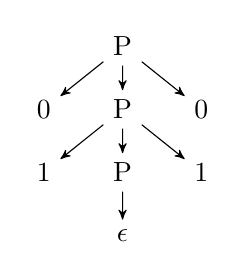
\begin{tikzpicture}[level distance=8mm,level/.style={sibling distance=10mm}]
  \node {P}
  child {node {0}}
  child {
    node {P}
    child {node {1}}
    child {
      node {P}
      child {node {\(\epsilon\)}}
    }
    child {node {1}}
  }
  child {node {0}};
\end{tikzpicture}
and get the \emph{yield} of the parse tree: \textbf{0110}
\section*{Un-ambiguous}
\emph{Ambiguous} grammar leads to \emph{un}-unique parse trees of a given string in language.  Techniques to remove ambiguity:
\begin{enumerate}
\item left/right associativity:
  \begin{itemize}
    \item[] change \(S \rightarrow S - S\) to
    \item \(S \rightarrow S - int\) [left assoc] or
    \item \(S \rightarrow int - S\) [right assoc]
  \end{itemize}
\item higher precedence: the \(V_{n}\) \textbf{closer} to \(V_{t}\) or use \verb|()|
  \begin{itemize}
    \item \(S \rightarrow S + T \gor T\) [lower]
    \item \(T \rightarrow T * \mathsf{int} \gor \mathsf{int}\) [lower]
    \end{itemize}
  \item[] \textbf{lower} level grammar productions have \textbf{higher} priority
  \item[] higher priority means the \textbf{break point} of a given string

\item Controlling \(\epsilon\):
  \vspace{-\baselineskip}
  \[
    S \rightarrow \epsilon \gor (S) \gor SS \Rightarrow\left\{
        \begin{array}{l}
          S \rightarrow \epsilon \gor T\\
          T \rightarrow TU \gor U\\
          U \rightarrow () \gor U \rightarrow (T)
        \end{array}
      \right.
  \]
  \vspace{-\baselineskip}
  % \begin{itemize}
  %   \item[] change \(S \rightarrow  \epsilon \gor (S) \gor SS\) to
  %   \item \(S \rightarrow \epsilon \gor T\)
  %   \item \(T \rightarrow TU \gor U\) and \(U \rightarrow () \gor (T)\)
  %   \item[] \(\epsilon\) can ONLY be derived from \(S\) and all other drvs go through T
  % \end{itemize}
\end{enumerate}
\section*{PDA}
\begin{itemize}
\item defines CFG and recognizes all and only the CFGs
\item essentially an \(\epsilon\)-NFA with an additional stack
\end{itemize}
\[ P = (Q,\Sigma,\Gamma,\delta,q_{0},Z_{0},F) \]
\begin{itemize}
\item[Q] finite set of \emph{states}
\item[\(\Sigma\)] finite set of \emph{input symbols}
\item[\(\Gamma\)] finite set of allowed \emph{stack alphabet}
\item[\(\delta\)] \emph{transition function} in the form: \(\delta(q,a,X)\)
  \begin{itemize}[leftmargin=1em,labelindent=2em]
  \item[$\delta$] is \emph{partial}: undefined for some input \(\notin \Sigma\)
  \item[$q$] a state \(\in Q\)
  \item[$a$] an input string of symbol(s) \(\in \Sigma\) or \(a = \epsilon\)
  \item[$X$] a stack symbol \(\in \Gamma \)
  \item[] Output a finite set of pairs \(p, \gamma\)
  \end{itemize}
\item[$q_{0}$] finite set of \emph{states}
\item[$Z_{0}$] finite set of \emph{states}
\item[$F$] finite set of \(accepting/final\; states \subseteq Q\)
\end{itemize}
\subsection*{PDA Trace and ID}
\begin{enumerate}[leftmargin=2.5em,labelindent=2em]
\item [same] \(\sigma(p,a,X) \rightarrow \{(q,X)\}\) (stack top unchanged)
\item [push] \(\sigma(p,a,X) \rightarrow \{(q,aX)\}\)
\item [pop]  \(\sigma(p,\epsilon,X) \rightarrow \{(q,\epsilon)\}\)
\end{enumerate}
\subsection*{Derive NPDA for CFG}
Given the CFG, derive its PDA using the following major steps
\begin{align*}
  S &\rightarrow S + T \gor T\\
  T &\rightarrow T * int \gor int
\end{align*}
\begin{enumerate}
\item \textbf{initialize} \(\delta(q_{0},\epsilon,Z) \mapsto q_{1}/SZ\)
\item \textbf{expand non-terminals}: input = \(\epsilon\) and expand stack top
  \begin{itemize}
  \item \(\delta(q_{1},\epsilon,S) \mapsto q_{1}/SZ\)
  \item \(\delta(q_{0},\epsilon,Z) \mapsto q_{1}/SZ\)
  \item \(\delta(q_{0},\epsilon,Z) \mapsto q_{1}/SZ\)
  \item \ldots
  \end{itemize}
\item \textbf{match and pop terminals}
\item \textbf{terminate}
\end{enumerate}

\subsection*{Trace}

\section*{Turing Machine (TM)}
\[
M = (Q,\Sigma,\Gamma,\delta,q_{0},B,F)
\]
\begin{itemize}
\item[$Q$] finite set of \emph{states} of finite control
\item[$\Sigma$] finite set of \emph{input symbols}: \(\Sigma \subset \Gamma\)
\item[$\Gamma$] complete set of \emph{tape symbols} and
\item[$\delta$] \emph{transition function}:
  \(
\delta\overbracket[1pt]{(q,X)}^\text{2 args} \overset{*}{\mapsto} \underbracket{(p,Y,D)}_\text{3 outputs}
  \)
  \begin{enumerate}
    \item \(q\) current state, \(q \in Q\)
    \item \(X\) current tape symbol, \(X \in \Gamma\)
    \item \(p\) next state, \(p \in Q\), from \(q\), through 0/more moves, to \(q\)
    \item \(Y \in \Gamma\), symb in tape cell, replacing whatever was there
    \item \(D\) \emph{direction}, \(L \leftarrow\), \(R \rightarrow\) or \(S\) (stay/halt)
 \end{enumerate}
\item[$q_{0}$] \emph{start state}: \(q_{0} \in Q\)
\item[$B$] \emph{blank} symbol, also \(\Lambda\)
\item[$F$] set of \emph{final} or \emph{accepting} states: \(F \subset Q\)
\end{itemize}
% Increment
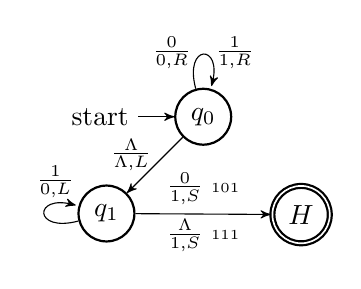
\begin{tikzpicture}[bezier bounding box]%reduce vertical space around graph
  \node[state, initial, minimum size=1em] (q0) {$q_0$};
  \node[state, minimum size=1em, below left=of q0] (q1) {$q_1$};
  \node[state, accepting, minimum size=1em, below right=of q0] (h) {$H$};

  \path[->] (q0)
  edge[loop above]
  node[yshift=-0.3cm,xshift=-0.4cm]{\footnotesize$\frac{0}{0,R}$}
  node[yshift=-0.3cm,xshift=0.4cm]{\footnotesize$\frac{1}{1,R}$} (q0)

  edge[above] node[yshift=-0.2cm,xshift=-0.3cm]{\footnotesize$\frac{\Lambda}{\Lambda,L}$} (q1)

  (q1) edge[loop left] node[yshift=0.4cm,xshift=0.5cm]{\footnotesize$\frac{1}{0,L}$}
  (q1) edge[above]
  node[yshift=-0.6cm]{\footnotesize$\frac{\Lambda}{1,S}$ \tiny111}
  node{\footnotesize$\frac{0}{1,S}$ \tiny101}(h);
\end{tikzpicture}
% Decrement
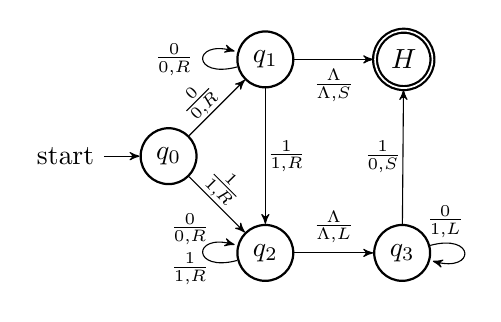
\begin{tikzpicture}[bezier bounding box]%reduce vertical space around graph
  \node[state, initial, minimum size=1em] (q0) {$q_0$};
  \node[state, minimum size=1em, above right=of q0] (q1) {$q_1$};
  \node[state, minimum size=1em, below right=of q0] (q2) {$q_2$};
  \node[state, minimum size=1em, right=of q2] (q3) {$q_3$};
  \node[state, accepting, minimum size=1em, right=of q1] (h) {$H$};

  \path[->]
  (q0)
  edge node[above,sloped,yshift=-0.1cm,xshift=-0.1cm]{\footnotesize$\frac{0}{0,R}$}(q1)
  edge node[above,sloped,yshift=-0.1cm,xshift=-0.1cm,]{\footnotesize$\frac{1}{1,R}$}(q2)

  (q1)
  edge[loop left] node{\footnotesize$\frac{0}{0,R}$}(q1)
  edge[below] node{\footnotesize$\frac{\Lambda}{\Lambda,S}$}(h)
  edge node[right,xshift=-0.1cm]{\footnotesize$\frac{1}{1,R}$}(q2)

  (q2)
  edge[loop left]
  node[yshift=0.3cm,xshift=0.2cm]{\footnotesize$\frac{0}{0,R}$}
  node[yshift=-0.2cm,xshift=0.2cm]{\footnotesize$\frac{1}{1,R}$}(q2)
  edge[above] node{\footnotesize$\frac{\Lambda}{\Lambda,L}$}(q3)

  (q3)
  edge[loop right] node[yshift=0.4cm,xshift=-0.6cm]{\footnotesize$\frac{0}{1,L}$}(q3)
  edge node[left,xshift=0.1cm]{\footnotesize$\frac{1}{0,S}$}(h);
\end{tikzpicture}
\(TM\) for inc binary num by 1 \hfill \(TM\) for dec binary num by 1
\subsection*{Lang of TM}
\(L(M)\) = set of all strings that halt \(M\) in its accepting state
\begin{itemize}
\item \textbf{total} TM halts for any given input (never stuck in loop)
\item \textbf{partial} TM halts for some input (loop forever)
\end{itemize}
\subsection*{Recursively Enumerable (RE)}
A lang is RE if \(L = L(M)\) for some TM \(M\)


\end{multicols*}
\end{document}
